A small square is constructed inside a square of area 1 by dividing each side of the unit square into $n$ equal parts, and then connecting the vertices to the division points closest to the opposite vertices.  Find the value of $n$ if the the area of the small square is exactly 1/1985.
\begin{center}
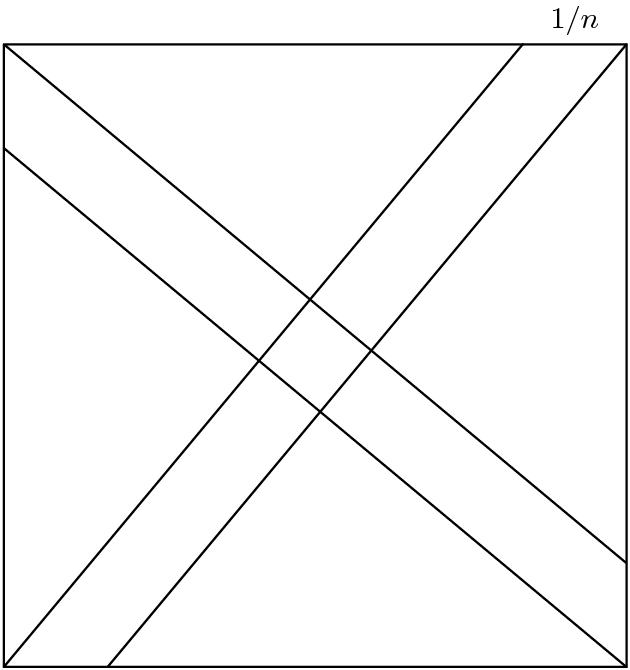
\includegraphics[width = 63.0mm]{img/fig0.png}
\end{center}